% This document is compiled using pdfLaTeX
% You can switch XeLaTeX/pdfLaTeX/LaTeX/LuaLaTeX in Settings

\documentclass{article}
% \usepackage[utf8]{inputenc}
\usepackage{graphicx}
\usepackage{float}
\usepackage{amssymb}

\title{Assignment 2}
\author{221300079 Juntong Wang}
\date{\today}

\begin{document}

	\maketitle

	\section{Question 1}
    In the lecture, we defined bisimulation for $\mathcal{ALC}$ and showed bisimulation invariance of $\mathcal{ALC}$ (Theorem 3.2).
    \begin{itemize}
        \item Define a notion of ``$\mathcal{ALCN}$-bisimulation'' that is appropriate for $\mathcal{ALCN}$ in the sense that bisimilar elements satisfy the same $\mathcal{ALCN}$-concepts.
        \item Use the definition to show that $\mathcal{ALCQ}$ is more expressive than $\mathcal{ALCN}$.
    \end{itemize}

    The Answer is followed:\\

    \textbf{Answer to item 1}:\\
    For answer to item 1, we need to extend the definition of Definition 3.1, we do the new $\mathcal{ALCN}$-bisimulation like this way:\\
    \begin{itemize}
        \item It inherits all the definition 3.1: the $\mathcal{ALC}$-bisimulation.
        \item If $d_1,d_2,...,d_n$ is the elements of domain $\Delta^{I_1}$ and such that every $(d,d_i) \in r^{I_1}$ for i from 1 to n is satisfiable, there are exist the same n elements $d_1',d_2',...,d_n'$ of domain $\Delta^{I_2}$ and such that every $(d',d_i') \in r^{I_2}$ for i from 1 to n is also satisfiable.
        \item If $d_1',d_2',...,d_n'$ is the elements of domain $\Delta^{I_2}$ and such that every $(d,d_i') \in r^{I_2}$ for i from 1 to n is satisfiable, there are exist the same n elements $d_1,d_2,...,d_n$ of domain $\Delta^{I_1}$ and such that every $(d,d_i) \in r^{I_1}$ for i from 1 to n is also satisfiable.
    \end{itemize}
    Here we gives out the correctness of the extend definition:\\
    Firstly, we consider an $\mathcal{ALCN}$ conception like:$C \equiv \leq(nr).\top$,for this then we get there is a d that $d \in (nr).^{I_1}$,so as the definition goes:\\
    iff there exists m which $m \leq n$,and $d_1, ...,d_m$ with $(d,d_i)\in r^{I_1}$\\
    So with the new definition 3.1 we get $d_1',...,d_m'$ with $(d,d_i')\in r^{I_2}$\\
    So we get $d' \in (nr).^{I_2}$\\
    So the symbal $C\equiv \geq (nr).\top$ is the same\\

    \textbf{Answer to item 2}\\
    As for this problem, we could construct the model and interpretation like this\\
    \begin{figure}[H]
        \centering
        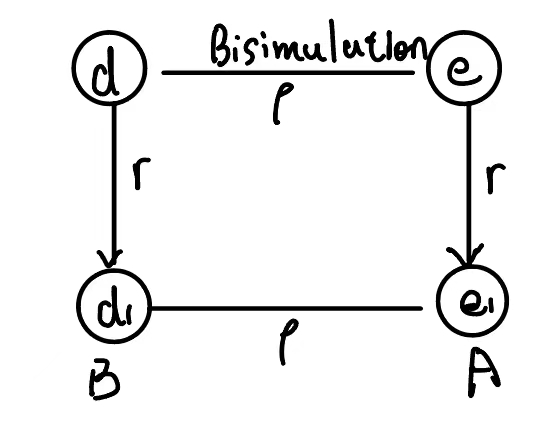
\includegraphics[width=0.8\textwidth]{1.png}\\
        \caption{bisimulation power}
        \label{fig:bisimulation}
    \end{figure}        
    If the $\mathcal{ALCN}$ and $\mathcal{ALCQ}$ like:$C\equiv \geq(1r).\top$ and $C\equiv \geq(1r).A$, for the former one it cannot distinguish the 2 bisimulation system, but the second one could distinguish them, for the left model it is false, but for the right model it is right. So we could prove that the  $\mathcal{ALCQ}$ is more expressive than $\mathcal{ALCN}$\\

    \section{Question 2}
    Let $C$ be an $\mathcal{ALC}$-concept, $\mathcal{T}$ an $\mathcal{ALC}$-TBox, $\mathcal{I}$ an interpretation and $\mathcal{J}$ its filtration w.r.t.\ $\textsf{sub}(C)\cup\textsf{sub}(\mathcal{T})$ (see Definition 3.14 for the definition of filtration). Show the truth or falsity of the following statement:
    \begin{itemize}
        \item the relation $\rho=\{(\textsf{d}, [\textsf{d}])~|~\textsf{d}\in\Delta^{\mathcal{I}}\}$ is a bisimulation between $\mathcal{I}$ and $\mathcal{J}$.
    \end{itemize}

    \textbf{The answer is as followed:false}\\
    Here is the reason:\\
    We do a little change of the example on class:let with the interpretation I, we have $A^I = \{d_1, d_2 ,d_1'\} \ B^I = \{d_2'\} \ R^I = \{(d_1,d_1'), (d_2, d_2')\}$,and we could have 
    if under the interpretation I, the situation is the left in the graph,and if we do the $S-Filtration$ we will get that $under \ interpretation \ J \ we \ have :[d_1]_s = [d_1']_s = \{d_1, d_1', d_2\}, [d_2']_s = \{d_2'\}$,so we have the graph 
    in the right place.So here we proved that the interpretation I and interpretation J they are fit for definition 3.15 but not fit the bisimulation $\rho$.\\
    \begin{figure}[H]
        \centering
        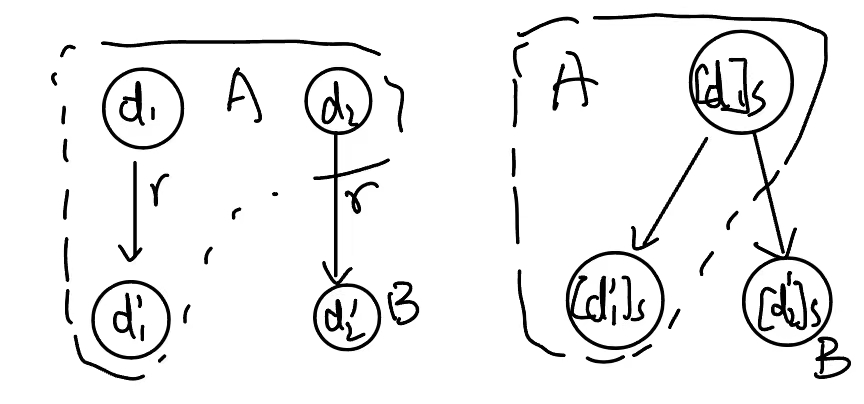
\includegraphics[width=0.8\textwidth]{2.png}\\
        \caption{An example not the bisimulation}
        \label{fig:bisimulation}
    \end{figure}  

    \section{Question 3}
    All the answer are followed the items\\
    We define ``\emph{bisimulations on $\mathcal{I}$}'' as bisimulations between an interpretation $\mathcal{I}$ and itself. Let $\textsf{d},\textsf{e}\in\Delta^{\mathcal{I}}$ be two elements. We write $\textsf{d}\approx_{\mathcal{I}}\textsf{e}$ if they are bisimilar, i.e., if there is a bisimulation $\rho$ on $\mathcal{I}$ such that $\textsf{d}~\rho~\textsf{e}$.
    \begin{itemize}
        \item Show that $\approx_{\mathcal{I}}$ is a bisimulation on $\mathcal{I}$.
        
        \textbf{Answer:}\\
        We only need do a little change according the problem and definition 3.1:\\
        (1)if $\textsf{d}\approx_{\mathcal{I}}\textsf{e}$ so we get there is an interpretation I such that $d \ \rho \ e$,
        which implies $d \in A^I\ iff\ e \in A^I for\ all\ A \in C$\\
        (2)if $\textsf{d}\approx_{\mathcal{I}}\textsf{e}$ and $(d,d') \in r^I$ so we get there is an interpretation I such that $d \ \rho \ e \ and\ (d,d') \in r^I$,
        which implies the existence of $e \in \Delta^I$ such that $d'\ \rho\ e' $ and $(e,e') \in r^I$ for all $r \in R$.So we could get $\textsf{d'}\approx_{\mathcal{I}}\textsf{e'}$,according to the definition in the problem.\\
        (3)only need to exchange the e and d in (2)\\
        So we have proved the $\approx_{\mathcal{I}}$ is bisimulation.\\  

    \end{itemize}
    Consider the interpretation $\mathcal{J}$ defined like the filtration, but with $\approx_{\mathcal{I}}$ instead of $\simeq$.
    \begin{itemize}
        \item Show that $\rho=\{(\textsf{d}, [\textsf{d}]_{\approx_{\mathcal{I}}})~|~\textsf{d}\in\Delta^{\mathcal{I}}\}$ is a bisimulation between $\mathcal{I}$ and $\mathcal{J}$.
        \textbf{Answer:}\\
        Before we prove it fit for the definition 3.1 we need take a little change on definition 3.14:\\
        \textbf{Define:}The equivalence class is $[\textsf{d}]_{\approx_{\mathcal{I}}} = \{e \in \Delta^I | \ \textsf{d}_{\approx_{\mathcal{I}}} \textsf{e}\}$\\
        \textbf{Define S-filtration:}\\
        \begin{itemize}
            \item $\Delta^J = \{[d]_{\approx_{\mathcal{I}}} | d \in \Delta^I\}$\\
            \item $A^J = \{[d]_{\approx_{\mathcal{I}}} | \exists d' \in [d]_{\approx_{\mathcal{I}}}.d' \in A^I\}$ for all $A \in C$\\
            \item $r^J = \{([d]_{\approx_{\mathcal{I}}},[e]_{\approx_{\mathcal{I}}})| \exists d' \in [d]_{\approx_{\mathcal{I}}}.(d',e') \in r^I \}$ for all $r \in R$\\ 
        \end{itemize}
        After that we start to prove the relation $\rho$ is bisimulation\\
        (1)Need to prove that $d \in \Delta^I iff [d]_{\approx_{\mathcal{I}}} \in A^J$:(Lemma 3.15)\\
        If $d \in A^I$ and there is $d \in [d]_{\approx_{\mathcal{I}}} \ so\ we\ get\ d {\approx_{\mathcal{I}}} d$so we get $d \in A^J$\\
        If $[d]_{\approx_{\mathcal{I}}} \in A^J$ so we could get there must be a $d' \in [d]_{\approx_{\mathcal{I}}}$, so according to the question above, we have show that the ${\approx_{\mathcal{I}}}$ is a bisimulation on I.\\
        So proved.\\
        (2)If we have $(d,[d]_{\approx_{\mathcal{I}}}) \in \rho$ and $(d,e) \in r^I$, so we get $d \in [d]_{\approx_{\mathcal{I}}}, e \in [e]_{\approx_{\mathcal{I}}},(d,e) \in r^I$ and according to (1) we get 
        $[d]_{\approx_{\mathcal{I}}}\in \Delta^J,[e]_{\approx_{\mathcal{I}}} \in \Delta^J$,so $(e,[e]_{\approx_{\mathcal{I}}} \in \rho)\ and\ ([d]_{\approx_{\mathcal{I}}},[e]_{\approx_{\mathcal{I}}}) \in \Delta^J$\\
        (3)So just go inverse of (2).\\
        So we get that the relation $\rho$ is a bisimulation between I and J\\

        \item Show that, if $\mathcal{I}$ is a model of an $\mathcal{ALC}$-concept $C$ w.r.t.\ an $\mathcal{ALC}$-TBox $\mathcal{T}$, then so is $\mathcal{J}$.\\
        \textbf{Answer:}\\
        If I is a model of an ALC-concept C with respect to an ALC-TBox $\tau$,according to definition 2.14, it is satisfiable, so it is not empty.\\
        And we get if $d \in C^I$, according to the bisimulation $\rho$, we get $[d]_{\approx_{\mathcal{I}}} \in C^J$\\
        And also according to the bisimulation between d and e, we let there is a GCI $D \sqsubseteq E$, so we get that $[d]_{\approx_{\mathcal{I}}} \in D^J$ so $[e]_{\approx_{\mathcal{I}}}\in D^J$, according to lemma 3.15 and also use the bisimulation
        we get $e \in D^I,e\in D^J,e\in E^J$,which implies the $[e]_{\approx_{\mathcal{I}}} \in E^J$\\
        So the model J of ALC-concept C with respect to an ALC-TBox $\tau$

        \item Why can't we use the previous result to show the finite model property for $\mathcal{ALC}$?\\
        \textbf{Answer:}\\
        We use the bisimulation to show some satisfiable and equivalence between interpretation I and interpretation J is fit.But we couldn't find a way
        that in the bisimulation to reduce the infinite models into the finite models.That means the J we constructed through the bisimulation also could be
        an infinite model, there is no restrict to the base of J.So we couldn't use the previous result to show the finite model property for ALC.\\

    \end{itemize}


    \section{Question 4}
    The answer is followed:\\
    Recall Theorem 3.8 from the lecture, which says that the disjoint union of a family of models of an $\mathcal{ALC}$-TBox $\mathcal{T}$ is again a model of $\mathcal{T}$. Note that the disjoint union is only defined for concept and role names.
    \begin{itemize}
        \item Extend the notion of disjoint union to individual names such that the following holds: for any family $(\mathcal{I}_{\nu})_{\nu\in\Omega}$ of models of an $\mathcal{ALC}$-knowledge base $\mathcal{K}$, the disjoint union $\biguplus_{\nu\in\Omega}\mathcal{I}_{\nu}$ is also a model of $\mathcal{K}$.\\
        
        \textbf{Answer:}\\
        According to definition 3.6, we get:
        \begin{itemize}
            \item $\Delta^J = \{(d,v)| v \in \Omega\ and\ d\ \in \Delta^{I_v}\}$
            \item $A^J = \{(d,v)| v \in \Omega\ and\ d\ \in A^{I_v}\}$ for all $A \in C$
            \item $r^J = \{((d,v),(e,v))| v \in \Omega\ and\ (d,e) \in r^{I_v}\}$for all $r \in R$      
            \item $a^J = \{(a,v)| holds\ like\ (a^{I_{v0}},v)\ for\ every\ individual\ under\ interpretation\ I_{v0}\}$
        \end{itemize}
        Also we get the knowledge base is consist of Tbox and Abox, so we prove it seperately.\\
        For Tbox:we firstly assume that J is not a model of TBox,so we get the GCIs:$C \sqsubseteq D $,so we get:
        $(d,v) \in \Delta^J$, so we get $(d,v)\in C^J\ and\ (d,v)\notin D^J$,so according to lemma 3.7 $d\in C^{I_v}\ and\ d\notin D^{I_v}$,so we get
        $I_v\ not\ \models  C \sqsubseteq D$ this is conflict to the satisfiable of model, so proved.\\
        For Abox:we firstly assume that J is not a model of Abox,so we get the assertion a:$(a^{I_v},v)\notin C^J$,so according to the bisimulation of $I_v and J$, we get that: $a^{I_v} \notin C^{I_v}$,which is not satisfiable for the model of K.
        Also the assertion $(a,b)$, we have $(a^{I_v},v),(b^{I_v},v) \notin C^J$ and we also get $(a^{I_v},v),(b^{I_v},v) \notin C^{I_v}$,also conflict with the definition of model K.\\
        So proved.\\
    \end{itemize}


    \section{Question 5}
    Let $\mathcal{K}=\{\mathcal{T}, \mathcal{A}\}$ be a consistent $\mathcal{ALC}$-KB. We write $C\sqsubseteq_{\mathcal{K}}D$ if $C^{\mathcal{I}}\subseteq D^{\mathcal{I}}$ holds for every model $\mathcal{I}$ of $\mathcal{K}$.
    \begin{itemize}
        \item Prove that for all $\mathcal{ALC}$-concepts $C$ and $D$ we have $C\sqsubseteq_{\mathcal{K}}D$ iff $C\sqsubseteq_{\mathcal{T}}D$.
        \textbf{Answer:}\\
        $\Leftarrow$:if we have $C\sqsubseteq_{\mathcal{T}}D$,according to the problem $K = \{T,A\}$,so with lemma 2.5 we get: every model of K is also the model of T, so proved.\\
        $\Rightarrow$:Because the $K = \{A,T\}$,we must have an interpretation $I_1$ which let the $C\sqsubseteq_{\mathcal{K}}D$ holds for it, and also $C\sqsubseteq_{\mathcal{T}}D$ holds for it.\\
        If we assume that there also an $I_2$ which let $C^{I_2} \nsubseteq  D^{I_2}$,and with the disjoint union J of $I_1\ and \ I_2$,we have the bisimulation $I_1$ and J, if they fit this we get:
        $(d,v) \in C^J,(d,v) \in D^J$,and we get $d \in C^{I_1},d \notin D^{I_2}$,this is conflict.So that $C^J \in D^J$,so we get the same with $I_2$ that $d\in C^{I_2},d\in D^{I_2}$. this is conflict with the assume. So proved.\\
    \end{itemize}


    \section{Question 6}
    All the answer is followed:\\
    Let $C$ be an $\mathcal{ALC}$-concept that is satisfiable w.r.t. an $\mathcal{ALC}$-TBox $\mathcal{T}$. Show truth or falsity of the following statement: 
    \begin{itemize}
        \item for all $m\geq 1$ there is a finite model $\mathcal{I}_{m}$ of $\mathcal{T}$ such that $|C^{\mathcal{I}_{m}}|\geq m$.\\
        \textbf{Answer:True}\\
        According to the problem,it is satisfiable, so as the finite model property goes:it must have a finite model I which fit $C^I \geq 1$;
        So if the $I_m = \biguplus_{i = 1,2,...,m} I_i$,so we have $C^{I_m} = m|C^i| \geq m$
        
        \item Does it hold if the condition ``$|C^{\mathcal{I}_{m}}|\geq m$'' is replaced by ``$|C^{\mathcal{I}_{m}}|=m$''?
        \textbf{Answer:False}\\
        According to the finite model property, if we replace it with the equivalence to m, it means for every I we have $C^I = 1$,we just need a anti-example to prove it is enough.\\
        This means we at least have 2 model in the interpretation I which is satisfiable for all GCIs.
        Here is an example:$A=\{\top\},GCIs=\{A \sqsubseteq \lnot \exists r.A,\lnot A \sqsubseteq \exists A\}$,for this two GCIs in the domain $\Delta^I$ we only have when both are empty are fit for them.
        So the for this interpretation the we have model $A = \emptyset,\lnot A = \emptyset $,so m is 2 not 1\\
    \end{itemize}

    \section{Question 7}
    Draw the unraveling of the following interpretation $\mathcal{I}$ at $d$ up to depth 5, i.e., restricted to $d$-paths of length at most 5 (see Definition 3.21):\\
    \textbf{Answer:}\\
    Here is the unraveling graph:\\
    \begin{figure}[H]
        \centering
        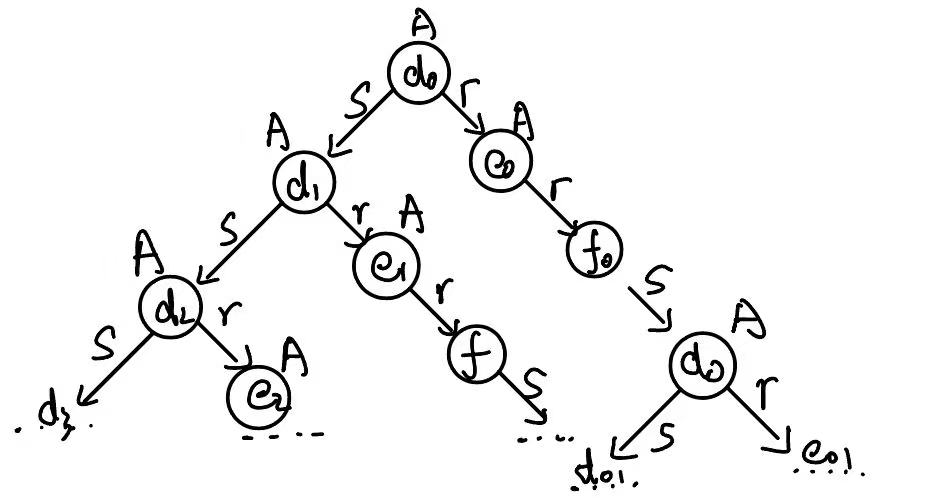
\includegraphics[width=1\textwidth]{3.png}\\
        \caption{Unraveling graph}
        \label{fig:Unraveling}
    \end{figure}  

    \section{Question 8}
    \begin{itemize}
        \item Show the truth or falsity of the following statement: if $\mathcal{K}$ is an $\mathcal{ALC}$-KB and $C$ an $\mathcal{ALC}$-concept such that $C$ is satisfiable w.r.t. $\mathcal{K}$, then $C$ has a tree model w.r.t. $\mathcal{K}$.\\
        \textbf{Answer:False}\\
        We could let the TBox as empty, and Abox be: $a:A,b:B,r:(a,b),(b,a)$.if A and B are two disjoint set, them it also satisfiable for the definition 2.14 and also it has a model like:$a->b->a$,so it is not a tree, it is a cycle. So the tree property not holds for the ALC-KB.
    \end{itemize}

    \section{Question 9}
    Interpretations of $\mathcal{ALC}$ can be represented as graphs, with edges labeled by roles and nodes labeled by sets of concept names. More precisely, in such a graph:
    \begin{itemize}
        \item[] each node corresponds to an element in the domain of the interpretation and it is labeled with all the concept names to which this element belongs in the interpretation;
        \item[] an edge with label $r$ between two nodes says that the corresponding two elements of the interpretation are related by the role $r$.
    \end{itemize}
    \begin{itemize}
    \item Show that: the description logic $\mathcal{S}$ (i.e., $\mathcal{ALC}$ with transitive roles) is more expressive than $\mathcal{ALC}$.\\
    \textbf{Answer:}\\
    \begin{figure}[H]
        \centering
        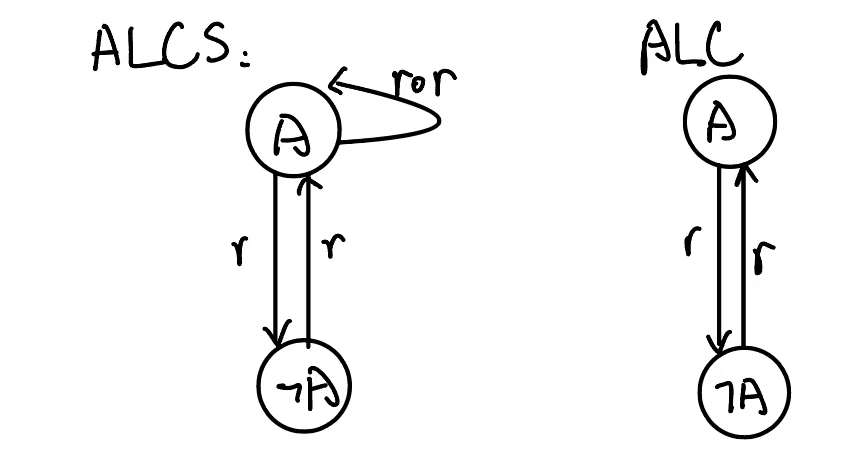
\includegraphics[width=1\textwidth]{4.png}\\
        \caption{Unraveling graph}
        \label{fig:Unraveling}
    \end{figure}  
    \end{itemize}
    Here we get the example,if we have ALC concepts:$A,\lnot A$,and TBox as $\{A \sqsubseteq \exists r.\lnot A, \lnot A \sqsubseteq \exists r.A\}$,in alc, we only have two relations so we get the A must be the $\emptyset$, but if we do this in ALCS concepts, we
    have the relation $A \sqsubseteq A$, so we have A is not just the $\emptyset$,it have a more powerful model expression, it's more expressive.\\
\end{document}


